\subsection{Charakteristik des Zählrohres}
Die Messergebnisse sind in der Tabelle \ref{tab:N/U} einzusehen.
In der Graphik \ref{fig:N/U} sind die Messwerte dargestellt.
\begin{table}[h!]
  \centering
  \caption{Ladung pro Teilchen}
  \label{tab:N/U}
  \begin{tabular}{c c c c c c c c c c c c c c}
    \toprule
      $U$/V & $I/\mu A$ &\Delta t /s & $N/\frac{1}{\text{min}}$ &$\sigma_N$&$Z/\frac{1}{s}$ &$\sigma_Z/\frac{1}{s}$& $Q/C\cdot10^{-10}$&$\sigma_Q\cdot10^{-10}$&$Q_{e0} \cdot 10^{10}$ & $\sigma_{Q_{e0}}\cdot10^9$\\
    \midrule
      300	& 0,0   & 60	& 0	    &   0	&   0,00    &  0,00   &    0,00 & 0,00 &  0,00 & 0,00\\
      310	& 0,05	& 60	& 9471	&  97	& 157,85	  &  1,62 	& 	 3,16	&	0,03 &	0,19 & 0,02\\
      320	& 0,1	  & 60	& 9940	&  99	& 165,66    &  1,66  	& 	 6,03	&	0,05 &	0,37 & 0,03\\
      330	& 0,1	  & 60	& 10011	& 100	& 166,85	  &  1,66 	& 	 5,99	&	0,05 &	0,37 & 0,03\\
      340	& 0,15	& 60	& 9963	&  99	& 166,05	  &  1,66 	& 	 9,03	&	0,08 &	0,56 & 0,05\\
      350	& 0,2	  & 60	& 10277	& 101	& 171,28    &  1,68  	& 	11,67	&	0,11 &	0,72 & 0,07\\
      360	& 0,2	  & 60	& 10365	& 101	& 172,75	  &  1,69 	& 	11,57	&	0,11 &	0,72 & 0,07\\
      370	& 0,2	  & 60	& 10254	& 101	& 170,90    &  1,68  	& 	11,70	&	0,11 &	0,73 & 0,07\\
      380	& 0,21	& 60	& 10406	& 102	& 173,43    &  1,70  	& 	12,10	&	0,11 &	0,75 & 0,07\\
      390	& 0,21	& 60	& 10228	& 101	& 170,46    &  1,68  	& 	12,31	&	0,12 &	0,76 & 0,07\\
      400	& 0,21	& 60	& 10238	& 101	& 170,63    &  1,68  	& 	12,30	&	0,12 &	0,76 & 0,07\\
      410	& 0,25	& 60	& 10330	& 101	& 172,16    &  1,69  	& 	14,52	&	0,14 &	0,90 & 0,08\\
      420	& 0,3	  & 60	& 10429	& 102	& 173,81    &  1,70  	& 	17,25	&	0,16 &	1,07 & 0,10\\
      430	& 0,38	& 60	& 10424	& 102	& 173,73    &  1,70  	& 	21,87	&	0,21 &	1,36 & 0,13\\
      440	& 0,4	  & 60	& 10475	& 102	& 174,58    &  1,70 	& 	22,91	&	0,22 &	1,43 & 0,13\\
      450	& 0,4	  & 60	& 10316	& 101	& 171,93    &  1,69 	& 	23,26	&	0,22 &	1,45 & 0,14\\
      460	& 0,4	  & 60	& 10583	& 102	& 176,38    &  1,71 	& 	22,67	&	0,21 &	1,41 & 0,13\\
      470	& 0,4	  & 60	& 10290	& 101	& 171,50    &  1,69  	& 	23,32	&	0,22 &	1,45 & 0,14\\
      480	& 0,41	& 60	& 10437	& 102	& 173,95	  &  1,70  	& 	23,56	&	0,22 &	1,47 & 0,14\\
      490	& 0,41	& 60	& 10358	& 101	& 172,63    &  1,69  	& 	23,74	&	0,23 &	1,48 & 0,14\\
      500	& 0,42	& 60	& 10427	& 102	& 173,78    &  1,70  	& 	24,16	&	0,23 &	1,50 & 0,14\\
      510	& 0,5	  & 60	& 10348	& 101	& 172,46    &  1,69 	& 	28,99	&	0,28 &	1,80 & 0,17\\
      520	& 0,5	  & 60	& 10606	& 102	& 176,76    &  1,71 	& 	28,28	&	0,27 &	1,76 & 0,16\\
      530	& 0,5	  & 60	& 10502	& 102	& 175,03    &  1,70 	& 	28,56	&	0,27 &	1,78 & 0,17\\
      540	& 0,55	& 60	& 10629	& 103	& 177,15	  &  1,71  	& 	31,04	&	0,29 &	1,93 & 0,18\\
      550	& 0,6	  & 60	& 10686	& 103	& 178,10    &  1,72  	& 	33,68	&	0,32 &	2,10 & 0,20\\
      560	& 0,65	& 60	& 10753	& 103	& 179,21    &  1,72  	& 	36,26	&	0,34 &	2,26 & 0,21\\
      570	& 0,65	& 60	& 10608	& 102	& 176,80    &  1,71 	& 	36,76	&	0,35 &	2,29 & 0,22\\
      580	& 0,65	& 60	& 10559	& 102	& 175,98    &  1,71  	& 	36,93	&	0,35 &	2,30 & 0,22\\
      590	& 0,7	  & 60	& 10402	& 101	& 173,36    &  1,69 	& 	40,00	&	0,39 &	2,52 & 0,24\\
      600	& 0,78	& 60	& 10635	& 103	& 177,25	  &  1,71  	& 	44,00	&	0,42 &	2,74 & 0,26\\
      610	& 0,78	& 60	& 10495	& 102	& 174,91    &  1,70  	& 	44,59	&	0,43 &	2,78 & 0,26\\
      620	& 0,78	& 60	& 10612	& 103	& 176,86    &  1,71  	& 	44,10	&	0,42 &	2,75 & 0,26\\
      630	& 0,8	  & 60	& 10675	& 103	& 177,91    &  1,72 	& 	44,96	&	0,43 &	2,80 & 0,26\\
      640	& 0,8	  & 60	& 10621	& 103	& 177,01    &  1,71 	& 	45,19	&	0,43 &	2,82 & 0,27\\
      650	& 0,82	& 60	& 10815	& 103	& 180,25	  &  1,73  	& 	45,49	&	0,43 &	2,83 & 0,27\\
      660	& 0,9	  & 60	& 10927	& 104	& 182,11    &  1,74 	& 	49,41	&	0,46 &	3,08 & 0,29\\
      670	& 0,9	  & 60	& 10704	& 103	& 178,40    &  1,72 	& 	50,00	&	0,48 &	3,14 & 0,30\\
      680	& 1,0	  & 60	& 10793	& 103	& 179,88    &  1,73 	& 	55,59	&	0,53 &	3,46 & 0,33\\
      690	& 1,0	  & 60	& 11083	& 105	& 184,71    &  1,75 	& 	54,13	&	0,50 &	3,37 & 0,31\\
      700	& 1,1	  & 60	& 11094	& 105	& 184,90    &  1,75  	& 	59,49	&	0,55 &	3,71 & 0,34\\
    \bottomrule
  \end{tabular}
\end{table}

\begin{figure}[h!]
  \centering
  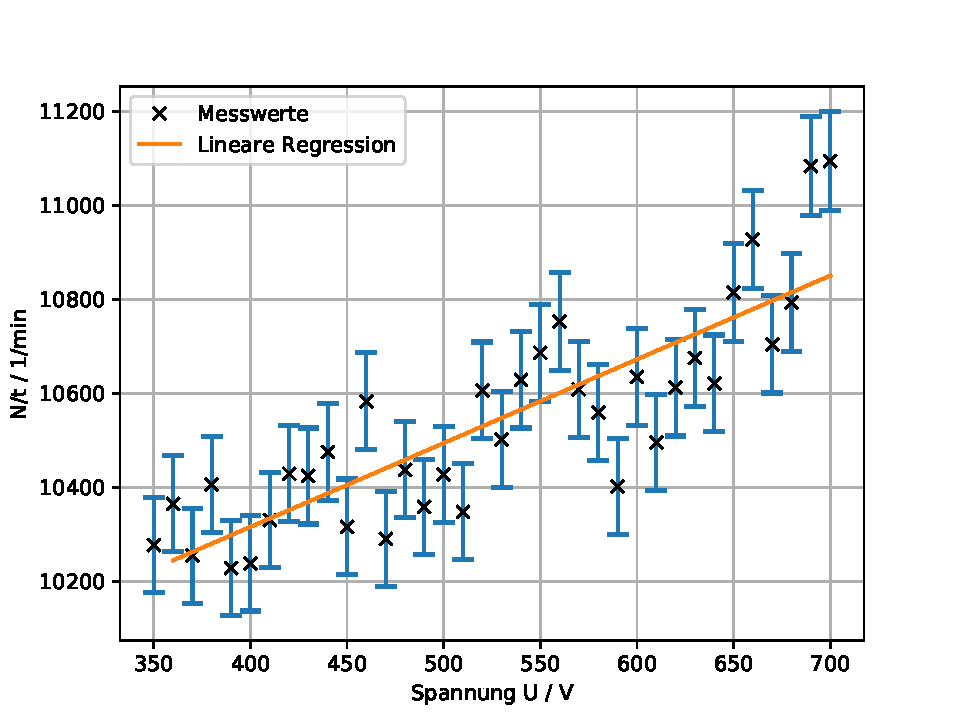
\includegraphics[width=\textwidth]{Graphik1.pdf}
  \caption{Charakteristik des Zählrohres}
  \label{fig:N/U}
\end{figure}

Für das Plateau wird eine lineare Ausgleichsrechnung durchgeführt.
Die Grade hat die Form:
\begin{align*}
  y=mx+b\\
  m=\SI{1,781\pm0,038}{\frac{1}{min V}}\\
  b=\SI{9603\pm97,995}{\frac{1}{min}}
\end{align*}
Die Steigung in Prozent beträgt: $m=\SI{4,17}{\percent}$ pro $\SI{100}{V}$.\\
Die Länge des Plateau reicht ungefähr von $\SI{320}{V}$ bis $\SI{680}{V}$.
\subsection{Bestimmung der Totzeit mit der Zwei-Quellen-Methode}
Bei $\SI{540}{V}$ werden zwei Unterscheidliche $\beta$-Quelle zusammen und getrent vermessen.
Es ergeben sich folgende Messwerte:
\begin{align*}
  N_{\text{R1}}&=\SI{10629\pm103}{\frac{1}{min}}\\
  N_{\text{R2}}&=\SI{1185\pm34}{\frac{1}{min}}\\
  N_{\text{R1+R2}}&=\SI{11642\pm108}{\frac{1}{min}}
\end{align*}
Mit der Formel \ref{eqn:T} lässt sich die Totzeit bestimmen.
\begin{align*}
  T\approx\SI{6,8\pm9,54e-6}{min}
\end{align*}
Der Fehler wird mit der Gauß'schen Fehlerfortpflanzung berechnet.
\begin{align*}
  \text{Fehler}=\sqrt{ \left(\frac{N_{\text{R2}}-N_{\text{R1+R2}}}{2N_{\text{R1}}^2N_{\text{R2}}}\right)^2\cdot(\SI{103}{})^2+\left(\frac{N_{\text{R1}}-N_{\text{R1+R2}}}{2N_{\text{R1}}N_{\text{R2}}^2}\right)^2\cdot(\SI{34}{})^2+\left(-\frac{1}{N_{\text{R1}}N_{\text{R2}}}\right)^2\cdot(\SI{108}{})^2}
\end{align*}

\subsection{Bestimmung der Totzeit mit Hilfe des Oszilloskops}
Für die Totzeitmessung mit dem Oszilloskop ergeben sich folgende Werte:
\begin{align*}
  T_{\text{U=460V}}&=3,8\cdot50\SI{}{\mu s}=\SI{3,17e-6}{min}\\
  T_{\text{U=510V}}&=4,0\cdot50\SI{}{\mu s}=\SI{3,33e-6}{min}\\
  T_{\text{U=580V}}&=4,2\cdot50\SI{}{\mu s}=\SI{3,5e-6}{min}
\end{align*}
\begin{figure}[h!]
  \centering
  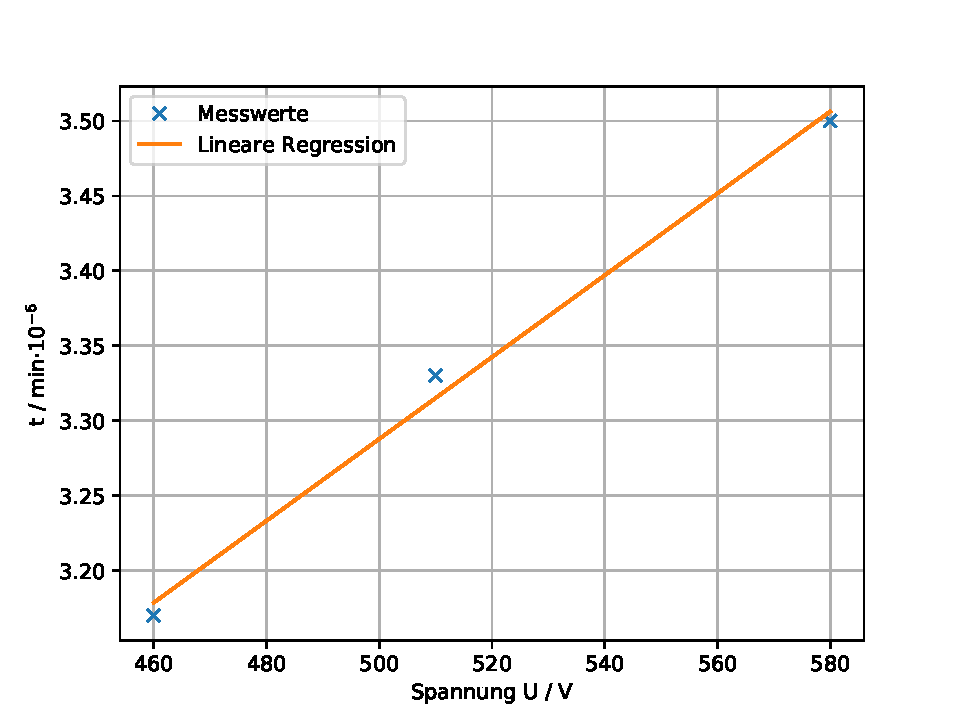
\includegraphics[width=\textwidth]{Totzeit2.pdf}
  \caption{Totzeitermittlung mit Hilfe des Oszilloskops}
  \label{fig:TotzeitOsz}
\end{figure}
Die Werte sind in der Graphik \ref{fig:TotzeitOsz} aufgetragen.
Mit einer Ausgleichsgraden der Form
\begin{align*}
  y&=ax+b\\
  a&=\SI{2,7\pm0,000046e-9}{\frac{min}{V}}\\
  b&=\SI{1,923\pm0,012e-6}{min}
\end{align*}
lässt sich für $T_{\text{U=540V}}=\SI{3,381\pm0,012e-6}{min}$ bestimmen.
Der Fehler wird mit der Gauß'schen Fehlerfortpflanzung berechnet.
\begin{align*}
  \text{Fehler}=\sqrt{ \left(x\right)^2\cdot(\SI{4,6e-14}{})^2+\left(1\right)^2\cdot(\SI{1,2e-8}{})^2}
\end{align*}

%%%%%%%%%%%%%%%%%%%%
%Jeder N Wert hat einen Feler von N^(1/2)
%Fehlerrechnug
Die Erholungszeit lässt sich nur grob abschätzen:
\begin{align*}
  T_{\text{U=460}}&=\SI{4e-6}{min}\\
  T_{\text{U=510}}&=\SI{1,17e-5}{min}\\
  T_{\text{U=580}}&=\SI{1,5e-5}{min}\\
  T_{\text{Mittelwert}}&=\SI{1,2e-5}{min}
\end{align*}

\subsection{Freigesetzte Ladung pro Teilchen}
Es wird der Strom in Abhängigkeit von der Spannung gemessen. Die Messergebnisse sind in der Tabell \ref{tab:N/U} zu finden.
Mit Hilfe der Formel \ref{eqn:I} kann der Strom pro Teilchen ausgerechnet werden. Das Z in der Formel ist die Anzahl der regestrierten Teilchen in der Zeit $\Delta T$.
Die Ergebnisse sind ebenfals in der Tabelle \ref{tab:N/U} dargestellt.
